\chapter{Crop Disease Prediction using Deep Learning}

\section{About}
Crop diseases are a major threat to food security, but their rapid identification remains difficult in many parts of the world due to the lack of the necessary infrastructure. The combination of increasing global smartphone penetration and recent advances in computer vision made possible by deep learning has paved the way for smartphone-assisted disease diagnosis. Using a public dataset~\cite{PlantVil94:online} of 54,306 images of diseased and healthy plant leaves collected under controlled conditions, we train a deep convolutional neural network to identify 14 crop species and 26 diseases (or absence thereof). Once the color coded image is overlaid on the Google Map, the farmer can go to the critical areas and click pictures of the unhealthy crops. These images will be evaluated against our already trained model and a prescription would be presented to the farmer on the application.

\section{Deep Learning Model}
Deep learning is a branch of machine learning based on a set of algorithms that attempt to model high level abstractions in data. In a simple case, you could have two sets of neurons: ones that receive an input signal and ones that send an output signal. When the input layer receives an input it passes on a modified version of the input to the next layer. In a deep network, there are many layers between the input and output (and the layers are not made of neurons but it can help to think of it that way), allowing the algorithm to use multiple processing layers, composed of multiple linear and non-linear transformations~\cite{deng2009imagenet}.

Many deep learning architectures such as Deep Neural Networks(DNNs), Convolutional Neural Networks(CNNs), and Recurrent Neural Networks(RNNs) have shown to produce state-of-the-art results on various tasks~\cite{ehler2006integrated}. As a powerful visual model, CNNs have demonstrated remarkable performance in various visual recognition problems, and attracted considerable attention in recent years.

The performance of convolutional neural networks in object recognition and image classification has made tremendous progress in the past few years. ~\cite{hughes2015open}, ~\cite{facts2015figures}, ~\cite{jia2014caffe}, ~\cite{krizhevsky2012imagenet} and ~\cite{lecun1989backpropagation}. Previously, the traditional approach for image classification tasks has been based on hand-engineered features such as SIFT~\cite{lecun2015deep}, HoG~\cite{lin2013network}, and then to use some form of learning algorithm in these feature spaces. This led to the performance of all these approaches depending heavily on the underlying predefined features. Feature engineering itself is a complex and tedious process which needed to be revisited every time the problem at hand or the associated dataset changed considerably. This problem has occurred in all traditional attempts to detect plant diseases using computer vision as they leaned heavily on hand-engineered features, image enhancement techniques, and a host of other complex and labour-intensive methodologies. 

\subsection{Convolutional Neural Networks}
Convolutional Neural Networks are very similar to ordinary Neural Networks, they are made up of neurons that have learnable weights and biases. Each neuron receives some inputs, performs a dot product and optionally follows it with a non-linearity. The whole network expresses a single differentiable score function: from the raw image pixels on one end to class scores at the other. And they have a loss function (e.g. SVM/Softmax) on the last (fully-connected) layer. CNN architectures make the explicit assumption that the inputs are images, which allows us to encode certain properties into the architecture. These then make the forward function more efficient to implement and vastly reduce the amount of parameters in the network~\cite{CS231nCo51:online}.


Neural Networks receive an input (a single vector), and transform it through a series of hidden layers. Each hidden layer is made up of a set of neurons, where each neuron is fully connected to all neurons in the previous layer, and where neurons in a single layer function completely independently and do not share any connections. The last fully-connected layer is called the ``output layer'' and in classification settings it represents the class scores, as it can be seen in Fig.~\ref{fig: extra-12} and Fig.~\ref{fig: extra-13}. Convolutional Neural Networks take advantage of the fact that the input consists of images and they constrain the architecture in a more sensible way. In particular, unlike a regular Neural Network, the layers of a CNN have neurons arranged in 3 dimensions: width, height, depth. 

\begin{figure}[h]
	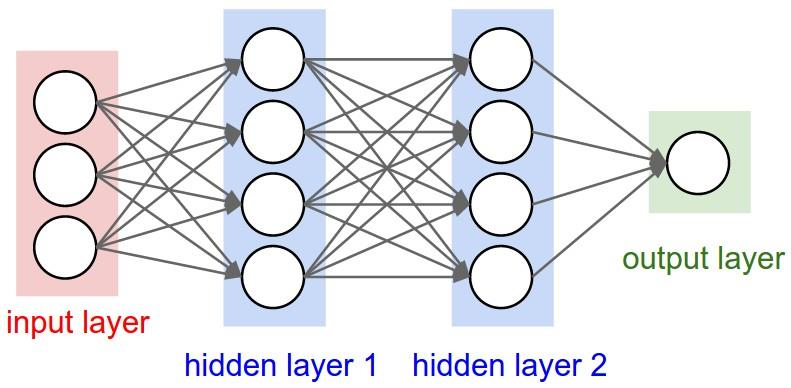
\includegraphics[width=1\linewidth]{extra-12}
	\centering
	\caption{\label{fig: extra-12}A regular 3-layer Neural Network~\cite{CS231nCo51:online}}
\end{figure}
\begin{figure}[h]
	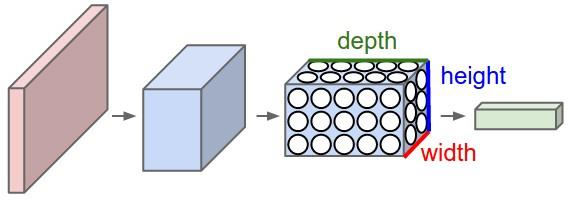
\includegraphics[width=1\linewidth]{extra-13}
	\centering
	\caption{\label{fig: extra-13}A CNN arranges its neurons in three dimensions (width, height, depth), as visualized in one of the layers. Every layer of a CNN transforms the 3D input volume to a 3D output volume of neuron activations. In this example, the red input layer holds the image, so its width and height would be the dimensions of the  image, and the depth would be 3 (Red, Green, Blue channels)~\cite{CS231nCo51:online}}
\end{figure}


A simple CNN is a sequence of layers, and every layer transforms one volume of activations to another through a differentiable function. We use three main types of layers to build CNN architectures: Convolutional Layer, Pooling Layer, and Fully-Connected Layer. In this way, CNNs transform the original image layer by layer from the original pixel values to the final class scores. 


\subsection{Deep Learning Frameworks}
Deep learning methods have resulted in significant performance improvements in several application domains and as such several software frameworks have been developed to facilitate their implementation to foster research and development in artificial intelligence. We can leverage these open-source tools and frameworks to implement many complex algorithms for different applications. Some of the very common frameworks include Caffe, Neon, TensorFlow, Theano, Torch, etc. 

Deep learning generally means building large scale neural networks with many layers. Simply put, these networks are simply functions which generate outputs Y given inputs X. In addition to the input X, the functions make use of a bunch of parameters (also called weights). These can include scalar values, vectors, and most expensively, matrices and higher-order tensors. A tensor is just a generalization of vectors and matrices into higher dimensions. The particular functions in vogue today involve tens of computationally expensive linear algebra operations, including matrix products and convolutions. Before we can train the network, we define a loss function. Common loss functions include squared error for regression problems and cross-entropy loss for classification. To train a network, we need to successively present many batches of new inputs to the network. After each is presented, we update the model by taking the derivative of the loss with respect to all of our parameters. So right away there are a few obvious problems. First, multiplying tens or hundreds or tensors together millions of times to process even a moderately sized dataset is terribly expensive. Second, taking the derivative of giant ugly functions by hand is a pain and could consume days or weeks that would be better spent imagining new experiments. This is why we need libraries like Theano, Caffe, Torch, and TensorFlow. The takeaway here is first that with any of these libraries you can write only the prediction code or forward pass and the framework will figure out how to take derivatives for you, that is to calculate the backwards pass. Second, you write your code once in a nice high-level language without ever learning the ugly details of GPU coding, and the framework will compile for whatever CPU or NVIDIA hardware you have access to.


\subsubsection{Why TensorFlow?}
TensorFlow is an open source software library by Google for numerical computation using data flow graphs. Nodes in the graph represent mathematical operations, while the graph edges represent the multidimensional data arrays (tensors) communicated between them. The flexible architecture allows us to deploy computation to one or more CPUs or GPUs in a desktop, server, or mobile device with a single API. The best part is that we can build every algorithm using easy to use data flow graphs which helps to visualize our algorithm’s architecture. TensorFlow seems to have a faster compile time and its computational graphs can be distributed on a cluster for computations. TensorFlow is both an R\&D and deployment framework. Support from such a huge company as Google is a big advantage for TensorFlow. TensorFlow can work with any gradient-based machine learning algorithm, which opens up a much broader range of uses. Written in C++ for speed, it doesn't require the developer to know anything about the underlying hardware. It also runs across multiple devices and architectures, so it's intended to scale from SoC devices, like phones, all the way up to distributed systems using dozens of GPUs. The main barrier to using any framework for math, statistics, or machine learning is ease-of-use. Likewise, one of TensorFlow's proffered advantages is ease-of-use. 

\textbf{Features:}


\begin{itemize}
	\item Multi GPU support
	\item Training across distributed systems
	\item Visualize the graphs using TensorBoard
	\item Model checkpointing
\end{itemize}


A few years ago, AlexNet~\cite{hughes2015open} showed for the first time that end-to-end supervised training using a deep convolutional neural network architecture is a practical possibility even for image classification problems with a very large number of classes, beating the traditional approaches using hand-engineered features by a substantial margin in standardbenchmarks. The absence of the labor-intensive phase of feature engineering and the generalizability of the solution makes them a very promising candidate for a practical and scalable approach for computational inference of plant diseases. Google also released its deep learning model GoogLeNet~\cite{szegedy2015going} in 2014 similar to AlexNet. Among the AlexNet and GoogLeNet architectures, GoogLeNet consistently performs better than AlexNet~\cite{mohanty2016using}, and based on the method of training, transfer learning always yields better results~\cite{mohanty2016using}, both of which were expected. An application of the ``network in network'' architecture~\cite{prince2015automatic} in the form of the inception modules is a key feature of the GoogleNet architecture.

In this report we used the concept of transfer learning to fine-tune the final layer of Google’s Inception V-3 (GoogLeNet) model based upon TensorFlow.

\subsection{Transfer Learning}
Modern object recognition models have millions of parameters and can take weeks to fully train. Transfer learning is a technique that shortcuts a lot of this work by taking a fully-trained model~\cite{pan2010survey} for a set of categories like ImageNet, and retrains from the existing weights for new classes. Transfer learning provides the opportunity to adapt a pre-trained model to new classes of data with several advantages. A basic concept of transfer learning is shown in Fig.~\ref{fig: transfer}.

\begin{figure}[h]
	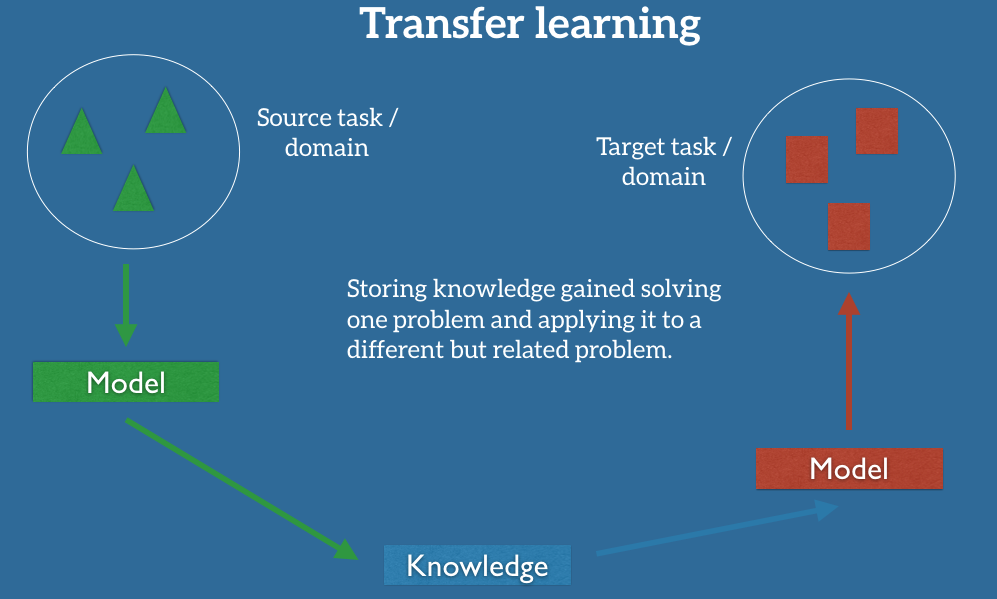
\includegraphics[width=1\linewidth]{fin_img_13}
	\centering
	\caption{\label{fig: transfer}Transfer Learning setup}
\end{figure}

In practice, we seek to transfer as much knowledge as we can from the source setting to our target task or domain. This knowledge can take on various forms depending on the data: it can pertain to how objects are composed to allow us to more easily identify novel objects; it can be with regard to the general words people use to express their opinions, etc. 

\subsubsection{Inception V-3 model}
Inception v3 is the 2015 iteration of Google’s Inception architecture for image recognition trained upon ImageNet data. Inception is a really great architecture and it’s the result of multiple cycles of trial and error.
 
Inception is basically:
\begin{itemize}
	\item An 299x299x3 input representing a visual field of 299 pixels
	and 3 color (RGB) channels
	\item Five vanilla convolution layers, with a few interspersed max-
	pooling operations
	\item Successive stacks of ``Inception Modules''
	\item A softmax ouput layer at the end ( logits ) and at an intermediate 	output layer ( aux\_logits ) just after the mixed 17x17x768e layer.
\end{itemize}


\begin{figure}[h]
	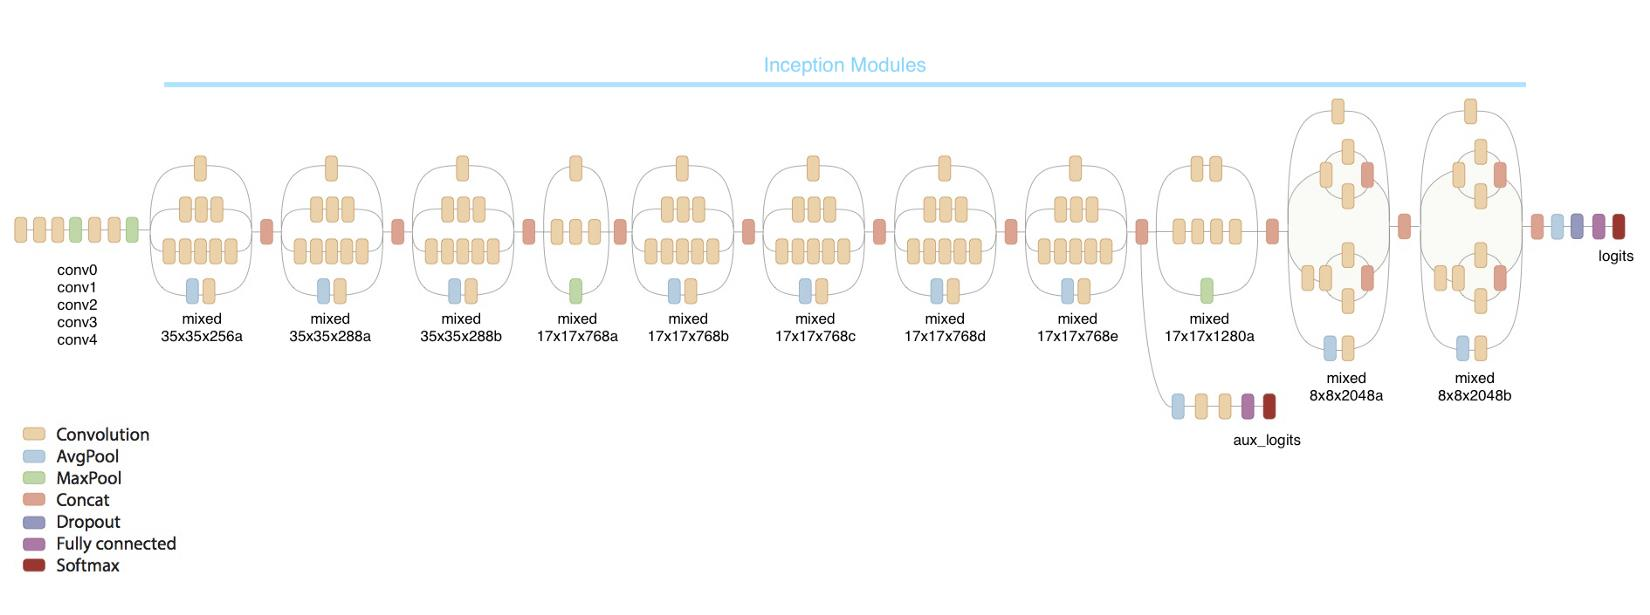
\includegraphics[width=1\linewidth]{fin_img_14}
	\centering
	\caption{\label{fig: inception}Overview of inception architecture~\cite{arxivorg71:online}}
\end{figure}




It’s the repeated stacking of the Inception modules that makes this architecture deep. While stacking Inception modules leads to depth, each module is also wide and architected to recognize features at multiple length scales. Overview of inception architecture is shown in Fig.~\ref{fig: inception}.











